% Converted from part_b_methods_results.md by scripts/md_to_latex.py; edit this file.
% DRAFT v0.1 (2026-10-07). Part B of the paper: wheel-size models, methods and results.
% Citations use Pandoc keys from ../references.bib, e.g. [@posirisuk2022].
% Build later with: pandoc part_b_methods_results.md --citeproc --bibliography ../references.bib -o part_b.docx
% Every number below is taken from outputs/ (paths given in the HTML comments) or from
% SIMULATION_METHODS.md. Re-check them if any simulation is rerun.
% Wheel sizes for the Voiager 5 are the reported 10/10 (stated assumption; see DOCUMENTATION.md 12).

\section{Methods: modelling the effect of wheel size}\label{methods-modelling-the-effect-of-wheel-size}

\subsection{Overview}\label{overview}

Rental e-scooters are the only e-scooters that may legally be ridden on UK public roads,
so a scooter with modified wheels cannot be tested on the road. We therefore used two
models, in the same way as the Imperial College study of e-scooter falls this work builds
on \autocite{posirisuk2022}:

\begin{enumerate}
\def\labelenumi{\arabic{enumi}.}
\tightlist
\item
  a \textbf{geometry model}, which describes how far a single wheel drops into a pothole and
  how hard it strikes the far edge, and
\item
  a \textbf{planar multibody dynamics model} of scooter and rider in MuJoCo
  \autocite{todorov2012mujoco}, which predicts whether the scooter pitches over.
\end{enumerate}

Both models compare wheel configurations under identical assumptions. They are not
validated against physical tests, so we report relative differences between
configurations, not real-world fall thresholds.

\subsection{Wheel configurations}\label{wheel-configurations}

Configurations are written front/rear diameter in inches (nominal size taken as tyre
outer diameter).

{\def\LTcaptype{none} % do not increment counter
\begin{longtable}[]{@{}
  >{\raggedright\arraybackslash}p{(\linewidth - 2\tabcolsep) * \real{0.5000}}
  >{\raggedright\arraybackslash}p{(\linewidth - 2\tabcolsep) * \real{0.5000}}@{}}
\toprule\noalign{}
\begin{minipage}[b]{\linewidth}\raggedright
Configuration
\end{minipage} & \begin{minipage}[b]{\linewidth}\raggedright
Meaning
\end{minipage} \\
\midrule\noalign{}
\endhead
\bottomrule\noalign{}
\endlastfoot
10/10 & Current vehicle (Voi Voiager 5, the model of all three ridden scooters as confirmed by Voi customer support \autocite{voi2026support_rec01,voi2026support_rec0203}), using the reported 10 in wheel size \autocite{levy_voiager5,alsalkini2023}; the front/rear split is not published, so equal wheels are assumed \\
12/10 & Larger front wheel only, as on Voi's Voiager 7 (12 in front) \autocite{startups2024voiager7} \\
12/12 & Larger wheels front and rear \\
14/10 & Much larger front wheel only \\
\end{longtable}
}

A front/rear ratio study added 16/10, 20/10, 16/8 and 20/8 (ratios up to 2.5).

\subsection{Geometry model}\label{geometry-model}

A rigid wheel of radius \(R\) rolls at speed \(v\) across a rectangular pothole of depth \(d\)
and length \(w\) with sharp edges. The wheel's lowest point sinks below road level by

\[h = \min\left(d,\; R - \sqrt{R^2 - (w/2)^2},\; \tfrac{1}{2} g \left(\tfrac{w}{v}\right)^2\right),\]

the smallest of the depth, the sag of a wheel resting on both edges, and the free-fall
distance in the time taken to cross (an upper bound). The far edge then meets the tyre at
an angle \(\theta\) from vertical, with \(\cos\theta = (R-h)/R\). Treating the impact as
plastic, the velocity lost into the edge is \(v\sin\theta\) and the forward speed loss of
the axle is \(v\sin^2\theta\). A larger wheel gives a smaller \(\theta\) for the same pothole,
so both quantities fall. Each wheel is analysed separately, so this model cannot say
whether the scooter falls; that requires the dynamics model.

The geometry model was evaluated for 8--16 in wheels, speeds of 15, 20 and 25 km/h,
depths of 0--120 mm and lengths of 150--1000 mm (\texttt{scripts/wheel\_geometry.py}).

\subsection{Dynamics model}\label{dynamics-model}

\textbf{Structure.} The model is planar (side view) with six degrees of freedom: forward
position, height and pitch of the chassis; rotation of each wheel; and forward lean of
the rider. It follows the structure of \textcite{posirisuk2022}, who modelled the scooter as the
front wheel and the rest of the scooter joined at the axle, but adds a separate rear
wheel, so that front-only and front-and-rear changes can be compared, and a rider. The
rider is a single rigid body pinned to the deck at the feet; a rotational spring
(1500 N·m/rad) and damper (150 N·m·s/rad) represent the rider bracing with legs and arms,
chosen so that braking at 0.3 g leans the rider about 8° forward.

\textbf{Parameters.} Voi does not publish the vehicle's mass properties, so most parameters
are assumed (Table~\ref{tab:4}). The rider's mass and height match the median male model of
\textcite{posirisuk2022}.

\begin{longtable}[]{@{}
  >{\raggedright\arraybackslash}p{(\linewidth - 4\tabcolsep) * \real{0.3333}}
  >{\raggedright\arraybackslash}p{(\linewidth - 4\tabcolsep) * \real{0.3333}}
  >{\raggedright\arraybackslash}p{(\linewidth - 4\tabcolsep) * \real{0.3333}}@{}}
\caption{Main model parameters.}\label{tab:4}\tabularnewline
\toprule\noalign{}
\begin{minipage}[b]{\linewidth}\raggedright
Parameter
\end{minipage} & \begin{minipage}[b]{\linewidth}\raggedright
Value
\end{minipage} & \begin{minipage}[b]{\linewidth}\raggedright
Source
\end{minipage} \\
\midrule\noalign{}
\endfirsthead
\toprule\noalign{}
\begin{minipage}[b]{\linewidth}\raggedright
Parameter
\end{minipage} & \begin{minipage}[b]{\linewidth}\raggedright
Value
\end{minipage} & \begin{minipage}[b]{\linewidth}\raggedright
Source
\end{minipage} \\
\midrule\noalign{}
\endhead
\bottomrule\noalign{}
\endlastfoot
Scooter mass & 32 kg & Assumed (Voiager 7 reported at 36 kg \autocite{startups2024voiager7}) \\
Wheel mass & 2.5 kg each & Assumed; scaling with diameter did not change results \\
Wheelbase & 0.95 m & Assumed \\
Deck height & 0.16 m (10 in wheels), rising with wheel size; deck kept level & Assumed \\
Handlebar height & 1.05 m & Assumed \\
Rider & 76 kg, 1.70 m, centre of mass at 55\% of height & \textcite{posirisuk2022}; centre-of-mass fraction assumed \\
Tyre compliance & Contact time constant 0.025 s (≈80 kN/m, ≈6 mm static deflection) & Assumed, typical small pneumatic tyre \\
Front fork & 25 kN/m, damping ratio 0.3, 30 mm travel & Assumed; the Voiager 5 has a front spring \autocite{levy_voiager5} \\
Friction & 0.9 & Dry asphalt, assumed \\
Integration & Implicit-fast, 0.5 ms time step & Numerical choice \\
\end{longtable}

\textbf{Tyre contact.} Wheels are rigid cylinders whose contact with the road is softened
through MuJoCo's soft-contact parameters to represent tyre compliance.

\textbf{Front suspension.} Because the Voiager 5 has a front spring, the main results use a
sprung front fork (Table~\ref{tab:4}). Its values were fixed before any run and tested in the
sensitivity analysis. Results without suspension are reported for comparison.

\textbf{Pothole.} The main experiments use a rectangular pothole with vertical walls and sharp
edges, 5 m after the start, giving about 1 s of run-up. To test potholes with broken
edges, a second contact model computes tyre--road contact directly against a sampled road
profile in which each edge falls over a width \(b\) with a raised-cosine shape (0, 25, 50 or
100 mm). It applies one radial spring-damper force per wheel. Before use, it was checked
on a flat road (0.01 g at the handlebar), for convergence with profile resolution, and
against MuJoCo's own contact on sharp edges, where fall outcomes agreed in 30 of 30 cases.
Its absolute accelerations are too high because a point contact cannot envelop an edge,
so it is used only to compare falls between edge shapes.

\textbf{Procedure.} Each run settles the model at rest for 0.5 s, sets the forward speed and
matching wheel spin, and lets the scooter coast (no motor or braking, no steering)
across the pothole.

\textbf{Outcomes.} Speed loss, maximum scooter pitch and rider lean, and peak acceleration at
the handlebar, where the phone was mounted. The handlebar acceleration is averaged over
10 ms windows to match the phone's 100 Hz sampling.

\textbf{Fall definition.} A run counts as a fall if the rider leans more than 30° forward,
the scooter pitches more than 30° nose-down, or forward speed drops below 0.5 m/s. These
thresholds are analyst-defined and were fixed before any experiment. A fall is attributed
to the rear wheel only if the rear wheel dipped more than 5 mm into the pothole before
the fall; otherwise it is attributed to the front-wheel impact.

\subsection{Experiments}\label{experiments}

\begin{longtable}[]{@{}
  >{\raggedright\arraybackslash}p{(\linewidth - 4\tabcolsep) * \real{0.3333}}
  >{\raggedright\arraybackslash}p{(\linewidth - 4\tabcolsep) * \real{0.3333}}
  >{\raggedright\arraybackslash}p{(\linewidth - 4\tabcolsep) * \real{0.3333}}@{}}
\caption{Simulation experiments.}\label{tab:5}\tabularnewline
\toprule\noalign{}
\begin{minipage}[b]{\linewidth}\raggedright
Experiment
\end{minipage} & \begin{minipage}[b]{\linewidth}\raggedright
Design
\end{minipage} & \begin{minipage}[b]{\linewidth}\raggedright
Runs
\end{minipage} \\
\midrule\noalign{}
\endfirsthead
\toprule\noalign{}
\begin{minipage}[b]{\linewidth}\raggedright
Experiment
\end{minipage} & \begin{minipage}[b]{\linewidth}\raggedright
Design
\end{minipage} & \begin{minipage}[b]{\linewidth}\raggedright
Runs
\end{minipage} \\
\midrule\noalign{}
\endhead
\bottomrule\noalign{}
\endlastfoot
Main sweep & 4 configurations × 9 depths (20--100 mm) × 3 lengths (300, 600, 1000 mm) × 3 speeds (15, 20, 25 km/h); with and without front suspension & 324 each \\
Sensitivity & Tyre stiffness (τ = 0.015, 0.035 s), rider bracing (1000, 3000 N·m/rad) and, with suspension, fork stiffness (15, 40 kN/m) and damping (ratio 0.15, 0.5), varied one at a time & 5 settings (9 with suspension) × 4 configurations \\
Front/rear ratio & 7 configurations from 10/10 to 20/8 on the main grid & 567 each \\
Soft edges & Profile contact with suspension; edge widths 0, 25, 50, 100 mm × main sweep & 1296 \\
Consistency check & 10/10 at 20 km/h on assumed common potholes (20--40 mm deep, 300 and 600 mm long) & 6 per model (with and without suspension) \\
\end{longtable}

The depth grid has a 10 mm resolution, so a reported threshold of ``80 mm'' means a first
fall somewhere between 70 and 80 mm. All runs are deterministic; rerunning the main sweep
and sensitivity analysis reproduced every outcome exactly. Analysis used NumPy, pandas
and Matplotlib \autocite{harris2020numpy,mckinney2010pandas,hunter2007matplotlib}; animations
were drawn with Matplotlib and encoded with Pillow \autocite{pillow}.

\textbf{Consistency check.} The criterion, fixed before running, was that simulated
handlebar peaks for the current scooter on common potholes should fall within roughly
1--3 g, the range of the measured impacts. With the three rides of Part A, 99 of 100
measured peaks were 1.0--2.97 g (median 1.27 g) and one was 6.28 g; the first ride alone
gave 1.0--2.8 g. Pothole depths along the route were not measured, so this is a
consistency check, not a validation.

\section{Results: what a larger front wheel would change}\label{results-what-a-larger-front-wheel-would-change}

\subsection{Geometry}\label{geometry}

At 20 km/h on a 600 mm long pothole, a 12 in front wheel reduced the edge impact
velocity by 6.5--7.7\% and the front-wheel speed loss by 12.6--14.8\% compared with a 10 in
wheel; a 14 in wheel reduced them by 12.1--13.9\% and 22.6--25.8\% (Table~\ref{tab:6}). At speed, wheels barely dropped
into short potholes (about 3 mm into a 150 mm pothole at 20 km/h), so long potholes are
the more dangerous ones.

% outputs/wheel_model/configurations.csv

\begin{longtable}[]{@{}
  >{\raggedright\arraybackslash}p{(\linewidth - 4\tabcolsep) * \real{0.3333}}
  >{\raggedright\arraybackslash}p{(\linewidth - 4\tabcolsep) * \real{0.3333}}
  >{\raggedright\arraybackslash}p{(\linewidth - 4\tabcolsep) * \real{0.3333}}@{}}
\caption{Front-wheel edge impact at 20 km/h, 600 mm pothole (geometry model).}\label{tab:6}\tabularnewline
\toprule\noalign{}
\begin{minipage}[b]{\linewidth}\raggedright
Front wheel
\end{minipage} & \begin{minipage}[b]{\linewidth}\raggedright
Depth 30 mm: impact velocity / speed loss
\end{minipage} & \begin{minipage}[b]{\linewidth}\raggedright
Depth 60 mm: impact velocity / speed loss
\end{minipage} \\
\midrule\noalign{}
\endfirsthead
\toprule\noalign{}
\begin{minipage}[b]{\linewidth}\raggedright
Front wheel
\end{minipage} & \begin{minipage}[b]{\linewidth}\raggedright
Depth 30 mm: impact velocity / speed loss
\end{minipage} & \begin{minipage}[b]{\linewidth}\raggedright
Depth 60 mm: impact velocity / speed loss
\end{minipage} \\
\midrule\noalign{}
\endhead
\bottomrule\noalign{}
\endlastfoot
10 in & 3.59 m/s / 41.7\% & 4.64 m/s / 69.8\% \\
12 in & 3.31 m/s / 35.5\% (−7.7\% / −14.8\%) & 4.34 m/s / 61.0\% (−6.5\% / −12.6\%) \\
14 in & 3.09 m/s / 30.9\% (−13.9\% / −25.8\%) & 4.08 m/s / 54.0\% (−12.1\% / −22.6\%) \\
\end{longtable}

At 60 mm and deeper, the drop is limited by the time available to fall (57 mm), so the
60 and 90 mm results are identical.

\begin{figure}[htbp]
\centering
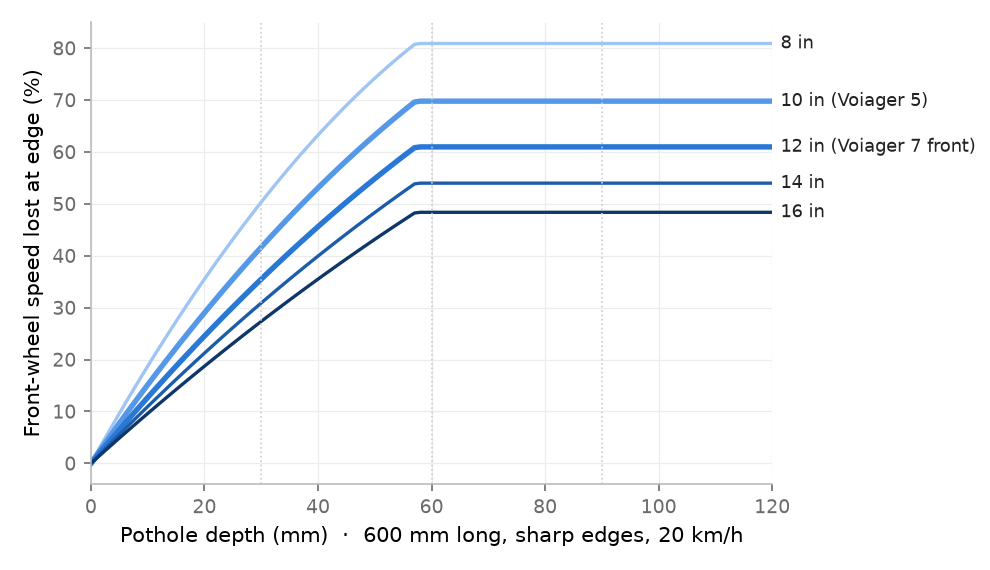
\includegraphics[width=\linewidth]{sim/geom_speed_loss.png}
\caption{Geometry model: share of the front wheel's speed lost at the far edge of a 600 mm long, sharp-edged pothole at 20 km/h, by wheel diameter. Rigid wheel, no tyre or suspension; the curves flatten at 57 mm, the deepest the wheel can drop in the time available. Schematic and further geometry results in Appendix~\ref{app:model}.}\label{fig:geom}
\end{figure}

Figure~\ref{fig:geom} shows the same comparison over all depths.

\subsection{Falls with the Voiager 5's front suspension}\label{falls-with-the-voiager-5s-front-suspension}

% outputs/scooter_sim/suspension/sim_results.csv, fall_thresholds.csv

With front suspension, falls occurred in 9 of 81 runs for the current 10/10
configuration, 6 for 12/10, 6 for 12/12 and 1 for 14/10 (Table~\ref{tab:7}). No 300 mm long
pothole caused a fall at any depth up to 100 mm; 600 mm potholes caused falls only at
15 km/h, where the slower wheel has more time to drop.

\begin{longtable}[]{@{}lllll@{}}
\caption{Shallowest pothole depth (mm) causing a fall, with front suspension (-- = no fall up to 100 mm). Rows with no falls in any configuration are omitted.}\label{tab:7}\tabularnewline
\toprule\noalign{}
Length, speed & 10/10 & 12/10 & 12/12 & 14/10 \\
\midrule\noalign{}
\endfirsthead
\toprule\noalign{}
Length, speed & 10/10 & 12/10 & 12/12 & 14/10 \\
\midrule\noalign{}
\endhead
\bottomrule\noalign{}
\endlastfoot
600 mm, 15 km/h & 80 & 90 & 90 & -- \\
1000 mm, 15 km/h & 90 & 100 & 100 & -- \\
1000 mm, 20 km/h & 90 & 90 & 90 & 100 \\
1000 mm, 25 km/h & 90 & 100 & 100 & -- \\
\textbf{Falls (of 81 runs)} & \textbf{9} & \textbf{6} & \textbf{6} & \textbf{1} \\
\end{longtable}

% outputs/scooter_sim/keyframes/keyframes_runs.csv

Figure~\ref{fig:5} shows one such case as still frames: the 80 mm deep, 600 mm long pothole at
15 km/h, the shallowest falling depth for the current scooter (Table~\ref{tab:7}). With 10 in
wheels the front wheel drops into the hole and strikes the far edge, and the scooter
pitches forward about it; the fall criterion is reached 0.15 s after the front wheel
reaches the edge. With a 12 in front wheel, alone or with a 12 in rear wheel, the
scooter rolls out with almost identical motion (maximum chassis pitch 13--14°,
speed loss 71--72\%). With a 14 in front wheel it rolls out with less pitch
(7°) and less speed loss (56\%).

\begin{figure}
\centering
{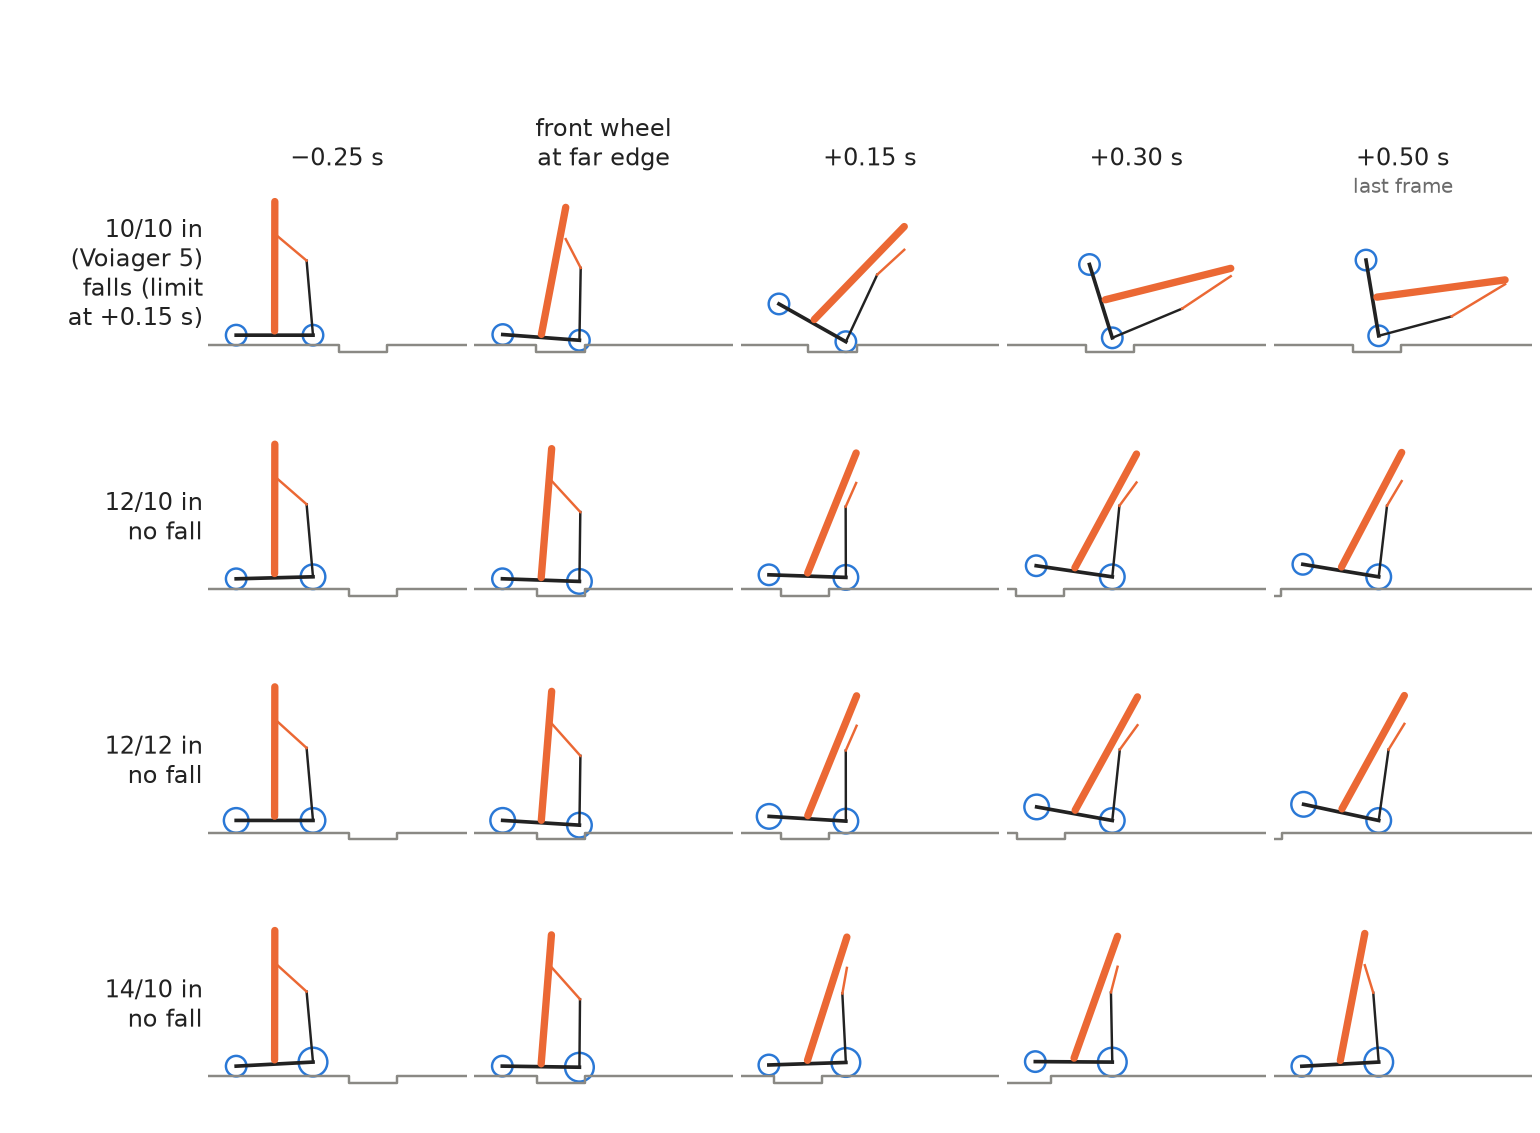
\includegraphics[width=\linewidth]{fig_b5_keyframes_sharp.png}}
\caption{Key frames from the simulation of the Voiager 5 model with its front spring
crossing a sharp-edged pothole 80 mm deep and 600 mm long at 15 km/h. Rows: wheel
configuration (front/rear diameter). Columns: the same moments in each row, relative to
the front wheel reaching the pothole's far edge; the view follows the front wheel. Blue:
wheels; black: deck and stem; orange: rider. The rider is pinned to the deck at the
feet, so scooter and rider rotate together; a real rider would separate from the scooter.
Planar model with assumed parameters (Table~\ref{tab:4}); one run per configuration, illustrating
the results of Table~\ref{tab:7}.}\label{fig:5}
\end{figure}

Every fall in every configuration was a forward pitch-over of scooter and rider about the
front wheel, started by the front-wheel impact; the rear wheel was lifted clear and never
entered the pothole before a fall. This matches the mechanism reported by
\textcite{posirisuk2022}.

The benefit of a 12 in front wheel was modest with suspension: it delayed the first fall
by 10 mm in three of the four cases above, and speed loss on a 60 × 600 mm pothole at
20 km/h was 25.5\% against 27.6\% for 10/10. A 14 in front wheel almost eliminated falls in
the tested range.

Without suspension, falls were more frequent (15, 14, 14 and 11 of 81 runs for 10/10,
12/10, 12/12 and 14/10), began at 70--80 mm for the current scooter, and the 12 in front
wheel delayed the fall by 10 mm on a 1000 mm pothole at 20 km/h (70 → 80 mm). The front
suspension itself therefore had a large effect, comparable to enlarging the front wheel.

\subsection{A larger front wheel alone performs like larger wheels front and rear}\label{a-larger-front-wheel-alone-performs-like-larger-wheels-front-and-rear}

The central comparison of the hypothesis is 12/10 against 12/12. In the main sweep they
had the same number of falls and the same shallowest falling depth in every case, both
with suspension (Table~\ref{tab:7}) and without. The reason is visible in the simulations: with
10--12 in wheels, the front-edge impact lifts the rear of the scooter so that the rear
wheel skips over the pothole, so its size makes almost no difference to whether the
scooter falls. In Figure~\ref{fig:5} the 12/10 and 12/12 rows are almost indistinguishable (speed
loss 70.9\% and 71.7\%).

\subsection{Sensitivity}\label{sensitivity}

% outputs/scooter_sim/sensitivity.csv, outputs/scooter_sim/suspension/sensitivity.csv

Without suspension, the 12/10 configuration fell at the same depth as 12/12, and 10 mm
deeper than 10/10, under all five tyre and bracing settings; the current scooter's
first fall on a 1000 mm pothole at 20 km/h moved between 60 and 70 mm with tyre
stiffness. With suspension, 12/10 and 12/12 fell at the same depth in 8 of 9 settings
(the exception, more fork damping, differed by 10 mm). The ordering of configurations was
therefore robust, but absolute fall depths depend on assumed parameters and should not be
read as real-world thresholds.

\subsection{Potholes without sharp edges}\label{potholes-without-sharp-edges}

% outputs/scooter_sim/suspension/soft_edges/edge_fall_counts.csv

\begin{longtable}[]{@{}lllll@{}}
\caption{Number of falls (of 81 runs) by edge width, profile contact with suspension.}\label{tab:8}\tabularnewline
\toprule\noalign{}
Edge width & 10/10 & 12/10 & 12/12 & 14/10 \\
\midrule\noalign{}
\endfirsthead
\toprule\noalign{}
Edge width & 10/10 & 12/10 & 12/12 & 14/10 \\
\midrule\noalign{}
\endhead
\bottomrule\noalign{}
\endlastfoot
0 mm (sharp) & 8 & 6 & 6 & 4 \\
25 mm & 8 & 5 & 6 & 4 \\
50 mm & 7 & 5 & 5 & 4 \\
100 mm & 4 & 3 & 3 & 2 \\
\end{longtable}

Sloped edges reduced falls (10/10: 8 to 4 from sharp to 100 mm edges). At every edge
width, the configurations with a larger front wheel fell less often than the current
scooter, and 12/10 stayed within one fall of 12/12. Figure~\ref{fig:6} shows the same 80 × 600 mm
pothole with 50 mm sloped edges: the current scooter still pitches over, more slowly
(fall criterion at 0.42 s), while 12 in and 14 in front wheels roll through. As with
sharp edges, 12/10 and 12/12 move almost identically (maximum chassis pitch 16°, speed
loss 50\%); 14/10 pitches less (11°, speed loss 44\%).

\begin{figure}
\centering
{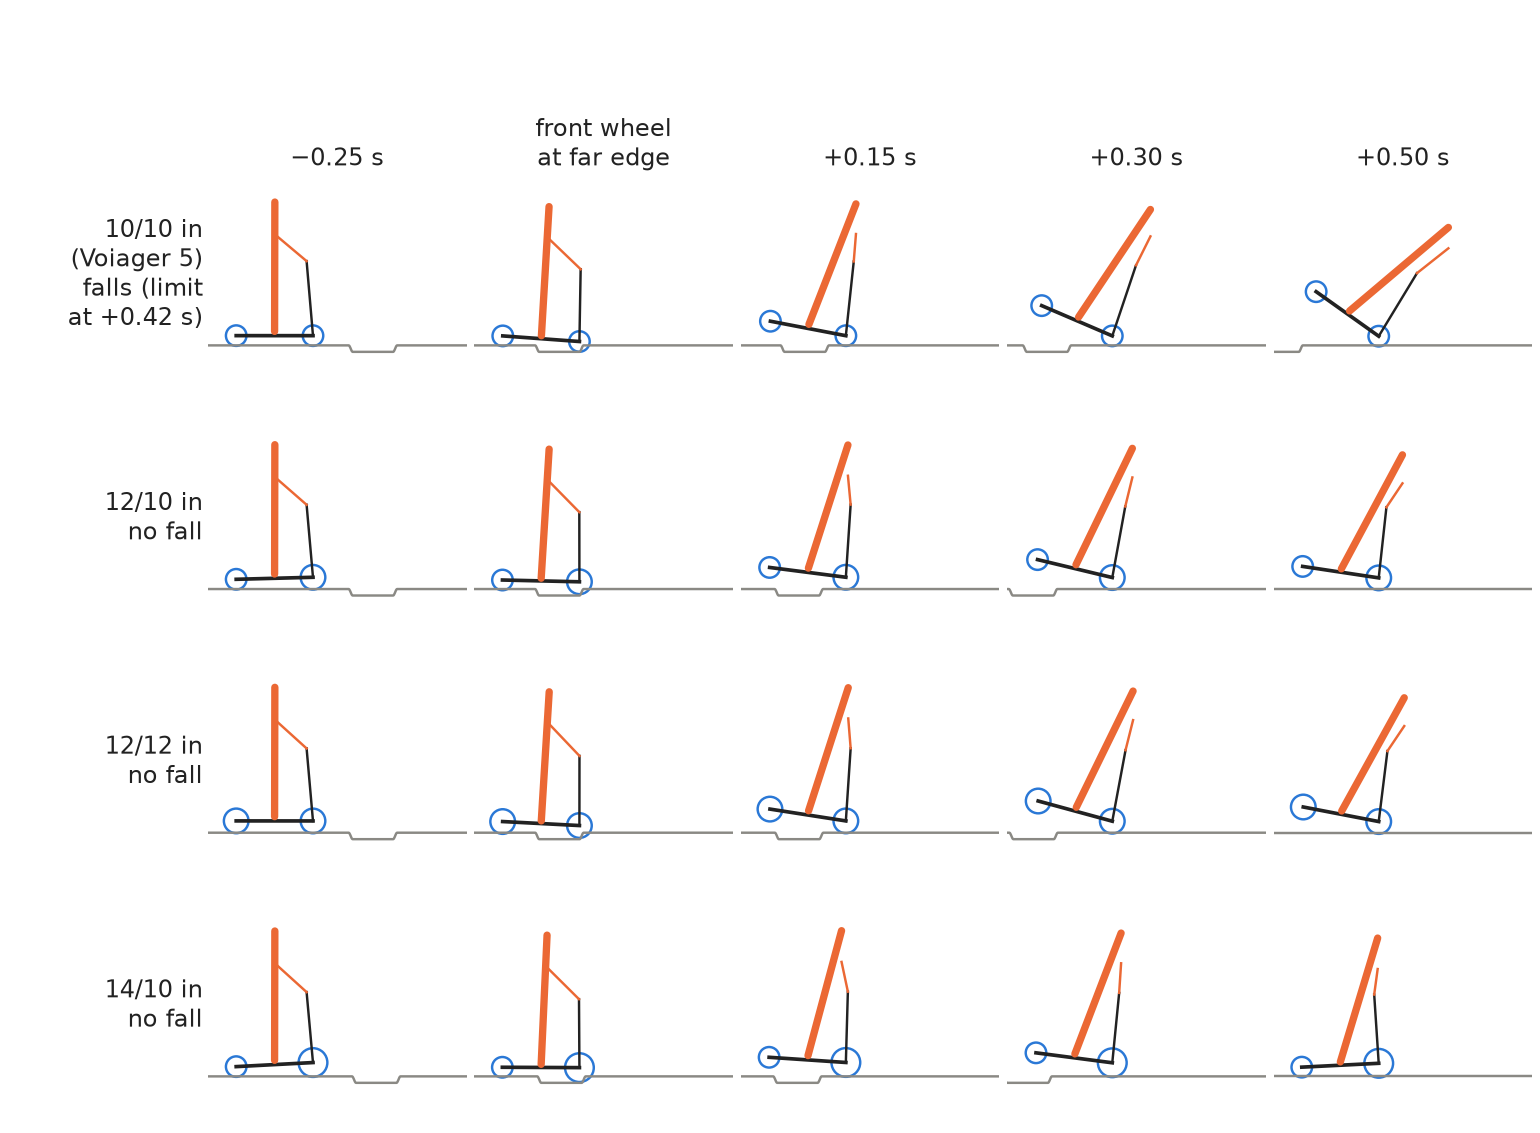
\includegraphics[width=\linewidth]{fig_b6_keyframes_edge50.png}}
\caption{As Figure~\ref{fig:5}, but each pothole edge slopes over 50 mm (raised-cosine profile,
custom tyre contact; section 3.4). Jolt sizes from
this contact model are not used as results; fall outcomes are.}\label{fig:6}
\end{figure}

\subsection{How much larger should the front wheel be?}\label{how-much-larger-should-the-front-wheel-be}

% outputs/scooter_sim/ratio/, outputs/scooter_sim/suspension/ratio/

The ratio study asked whether a front wheel can be too large relative to the rear. It
repeated the main sweep (81 runs per configuration) for front/rear diameter ratios from
1.0 (10/10) to 2.5 (20/8); the full results are in Appendix~\ref{app:ratio}. Falls kept
decreasing as the front wheel grew (Table~\ref{tab:9}): from 15 of 81 runs for 10/10 to 1
for 20/10 and 20/8 without suspension, and from 9 to none with suspension. No ratio up
to 2.5 made falls more likely: with a larger front wheel the shallowest depth causing a
fall stayed the same or rose, in 10 mm steps (Figures~\ref{fig:Eratiofork} and~\ref{fig:Erationofork}).

% outputs/scooter_sim/ratio/ratio_results.csv, outputs/scooter_sim/suspension/ratio/ratio_results.csv
\begin{table}[htbp]
\centering\small
\caption{Front/rear ratio study: runs meeting the fall criteria (of 81 per configuration). Planar model with assumed parameters (Table~\ref{tab:4}); relative comparison of wheel configurations only.}\label{tab:9}
\begin{tabular}{@{}lrrr@{}}
\toprule
Front/rear (in) & Ratio & Without suspension & With suspension \\
\midrule
10/10 & 1.0 & 15 & 9 \\
11/10 & 1.1 & 15 & 9 \\
12/10 & 1.2 & 14 & 6 \\
14/10 & 1.4 & 11 & 1 \\
16/10 & 1.6 & 9 & 1 \\
20/10 & 2.0 & 1 & 0 \\
16/8 & 2.0 & 9 & 1 \\
20/8 & 2.5 & 1 & 0 \\
\bottomrule
\end{tabular}
\end{table}


Very large front wheels did change what the rear wheel does (Figures~\ref{fig:Erearfork}
and~\ref{fig:Erearnofork}). With a small front wheel, the front impact lifts the rear so
that it skips over the pothole. With a very large front wheel it no longer does, so the
rear wheel drops into the pothole and causes a second jolt: without suspension, the
largest speed loss at the rear crossing (20 km/h, runs without a fall) rose from 19\% for
10/10 to 27\% for 20/10 and 33\% for 20/8. With suspension the configurations differed
little. This second jolt caused no falls in the model, but it would affect comfort and
control.

In this model a larger front wheel was never worse: falls kept decreasing up to the
largest front wheel tested (20 in). With front suspension, however, most of the reduction
was reached by 14/10 (from 9 to 1 of 81 runs), and larger front wheels added little. The
model cannot represent steering, frame geometry, weight or cost, all of which limit how
large a front wheel can practically be, and the rear-wheel jolt above would affect
comfort. We therefore suggest a moderate increase (12--14 in), in line with wheels already
in use: the Voiager 7 has a 12 in front wheel \autocite{startups2024voiager7}, and London's
tender requires a front wheel of at least 11 in \autocite{tfl2022tender}. This limit is a
judgement based on factors outside the model, not a result of it.

\subsection{Consistency with the measured rides}\label{consistency-with-the-measured-rides}

% outputs/scooter_sim/consistency.csv; measured: outputs/combined/impacts_all.csv

With front suspension, simulated handlebar peaks for the current scooter on 300 mm long
potholes were 1.9--2.4 g, inside the range of 99 of the 100 measured impacts
(1.0--2.97 g). On 600 mm potholes they were 4.2--5.7 g, about twice that range; only one
measured impact (6.28 g) was higher, and a single value is not taken as agreement.
Without suspension they were 4.9--9.8 g, three to five times too high. The suspension model is therefore the more
faithful representation of the Voiager 5 and is used for the main results, with the
caveat that its absolute accelerations are reliable only for short potholes.
 Figure~\ref{fig:consistency} shows the comparison.

\begin{figure}[htbp]
\centering
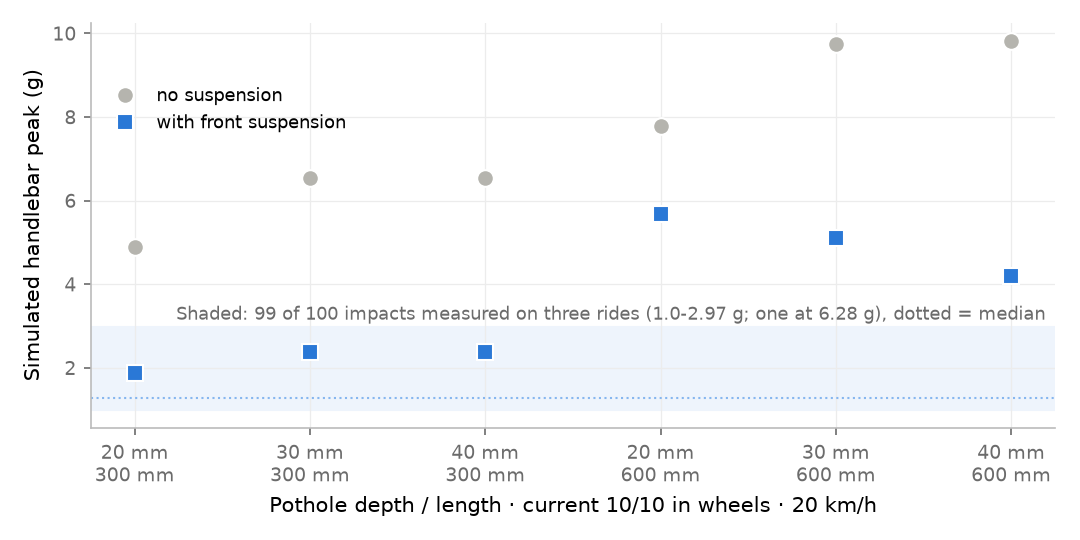
\includegraphics[width=\linewidth]{sim/consistency.png}
\caption{Consistency check: simulated handlebar peaks for the current 10/10 configuration at 20 km/h, with and without front suspension, against the range of 99 of the 100 impacts measured on the three rides (shaded; dotted line: median). Pothole depths on the route were not measured, so this is a consistency check, not a validation.}\label{fig:consistency}
\end{figure}

\subsection{Limitations of the models}\label{limitations-of-the-models}

\begin{itemize}
\tightlist
\item
  \textbf{Planar:} no steering, handlebar twist, roll or sideways falls. Loss of steering
  control, which a front-wheel impact can also cause, is not represented.
\item
  \textbf{Assumed vehicle:} mass, inertias, wheelbase, tyre stiffness, fork and the rear wheel
  size are not published by Voi.
\item
  \textbf{Simple rider:} one rigid body with a fixed spring; no active balance or reaction.
\item
  \textbf{Idealised potholes:} rectangular, or with smooth sloped edges; real potholes are
  irregular.
\item
  \textbf{Potholes only:} other obstacles were not part of the main study. An exploratory
  extension to raised bumps (Appendix~\ref{app:bumps}) found the same benefit of a larger
  front wheel without suspension, but with the front spring the few modelled bump falls
  started at the rigid rear wheel, so the front-wheel result may not hold for every type of
  obstacle.
\item
  \textbf{Analyst-defined falls} and a 10 mm depth resolution.
\item
  \textbf{Not validated} against physical tests; the consistency check is only a partial pass.
\end{itemize}

Within these limits, the models consistently show that the front wheel determines whether
the scooter pitches over, and that enlarging the front wheel alone gives the same benefit
in the model as enlarging both wheels.
